\section{Introduction}
%Each section needs a subsection for the small points on top to show up
\subsection{Dummy}

\begin{frame}{Overview}
Quasicrystals: ordered, aperiodic materials $\to$ Bloch's theorem fails.

\textbf{Today's goal}: construct non-interacting tight-binding electronic eigenstates from geometrical \emph{height fields}.

Pioneering work (reverse engineered toy model):
\begin{itemize}
	\item {\ss{Self-similar ground-state wave function for electrons on a 2D Penrose lattice}\\\emph{Sutherland, PRB 34 (6), 1986}}
\end{itemize}
Breakthrough (reasonable toy model):
\begin{itemize}
	\item {\ss{Electrons in deterministic quasicrystalline potentials and hidden conserved quantities}\\\emph{Kalugin, Katz, J. Phys. A 47 (31), 2014}}
\end{itemize}
A ``pedagogical'' version of the previous paper:
\begin{itemize}
	\item {\ss{Critical eigenstates and their properties in one-and two-dimensional quasicrystals}\\
	\emph{Macé, Jagannathan, Kalugin, Mosseri, Piéchon, PRB 96 (4), 2017}}
\end{itemize}

Many thanks to Michel Duneau, Jean-Noël Fuchs, Jean-Marc Luck, Éric Akkermans.
\end{frame}

\section{Quasiperiodic geometry}
\subsection{Dummy}
\begin{frame}{Periodic, quasiperiodic and random}
\only<1>{
A random tiling:

\centering
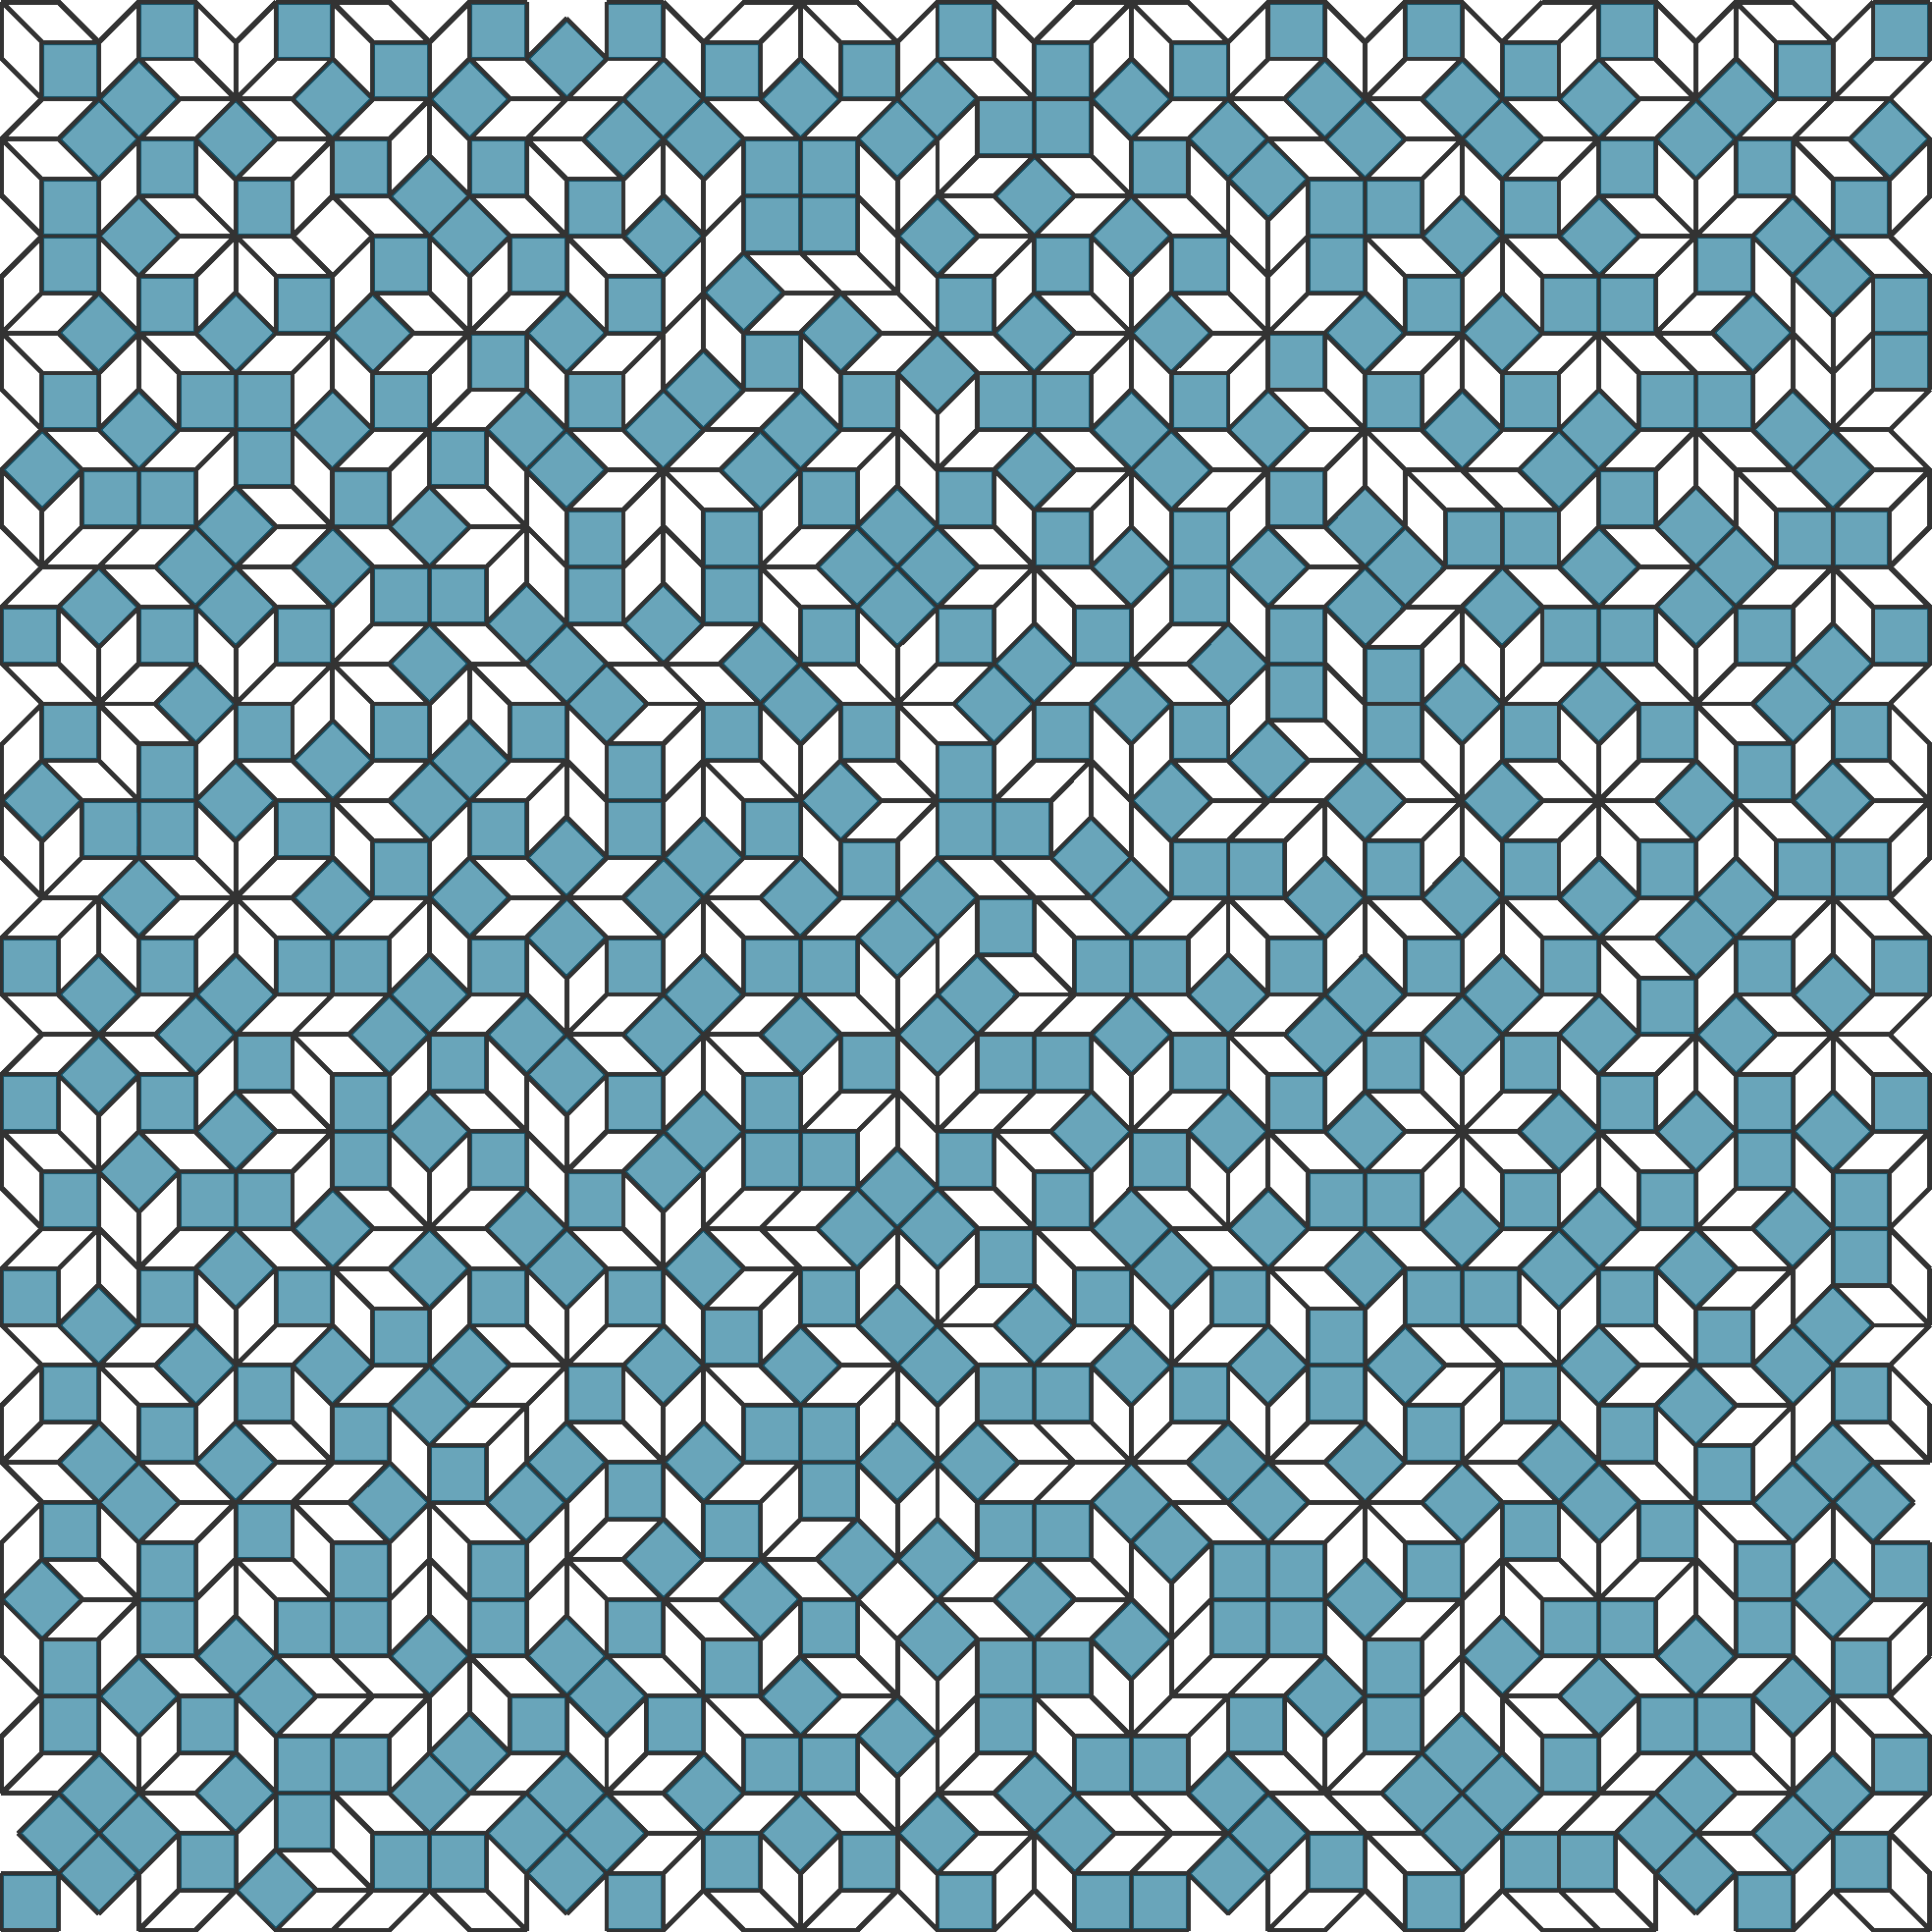
\includegraphics[width=.5\textwidth]{img/random00.pdf}

}

\only<2>{
Two copies of the tiling:

\centering
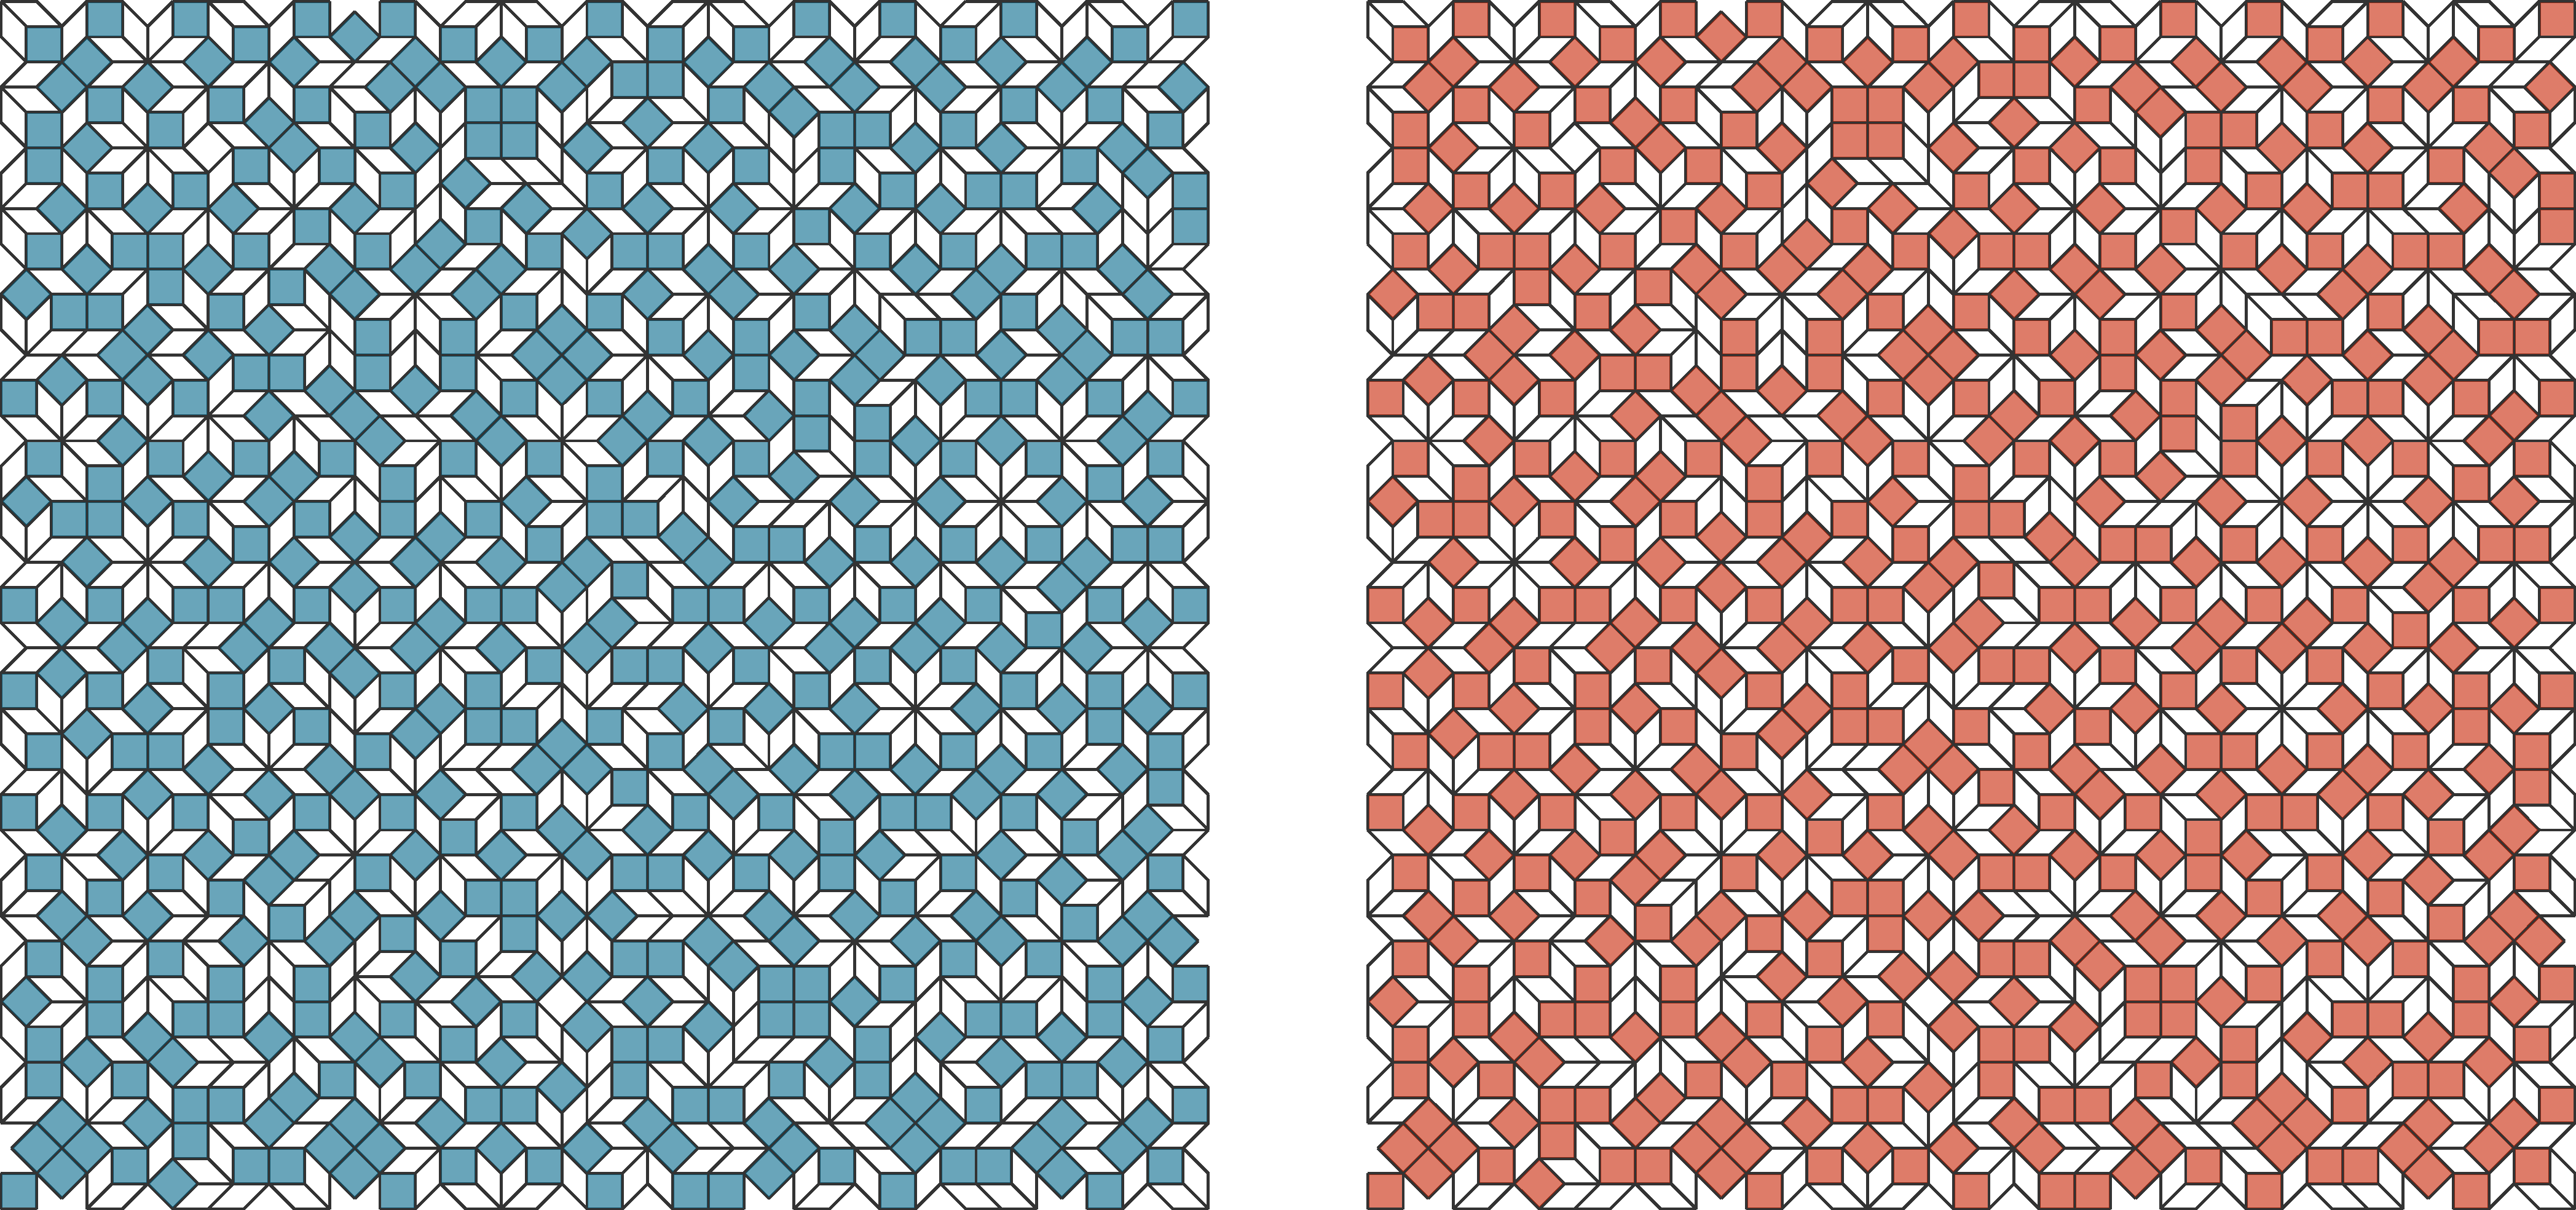
\includegraphics[width=1.\textwidth]{img/random01.pdf}

}

\only<3>{
\centering
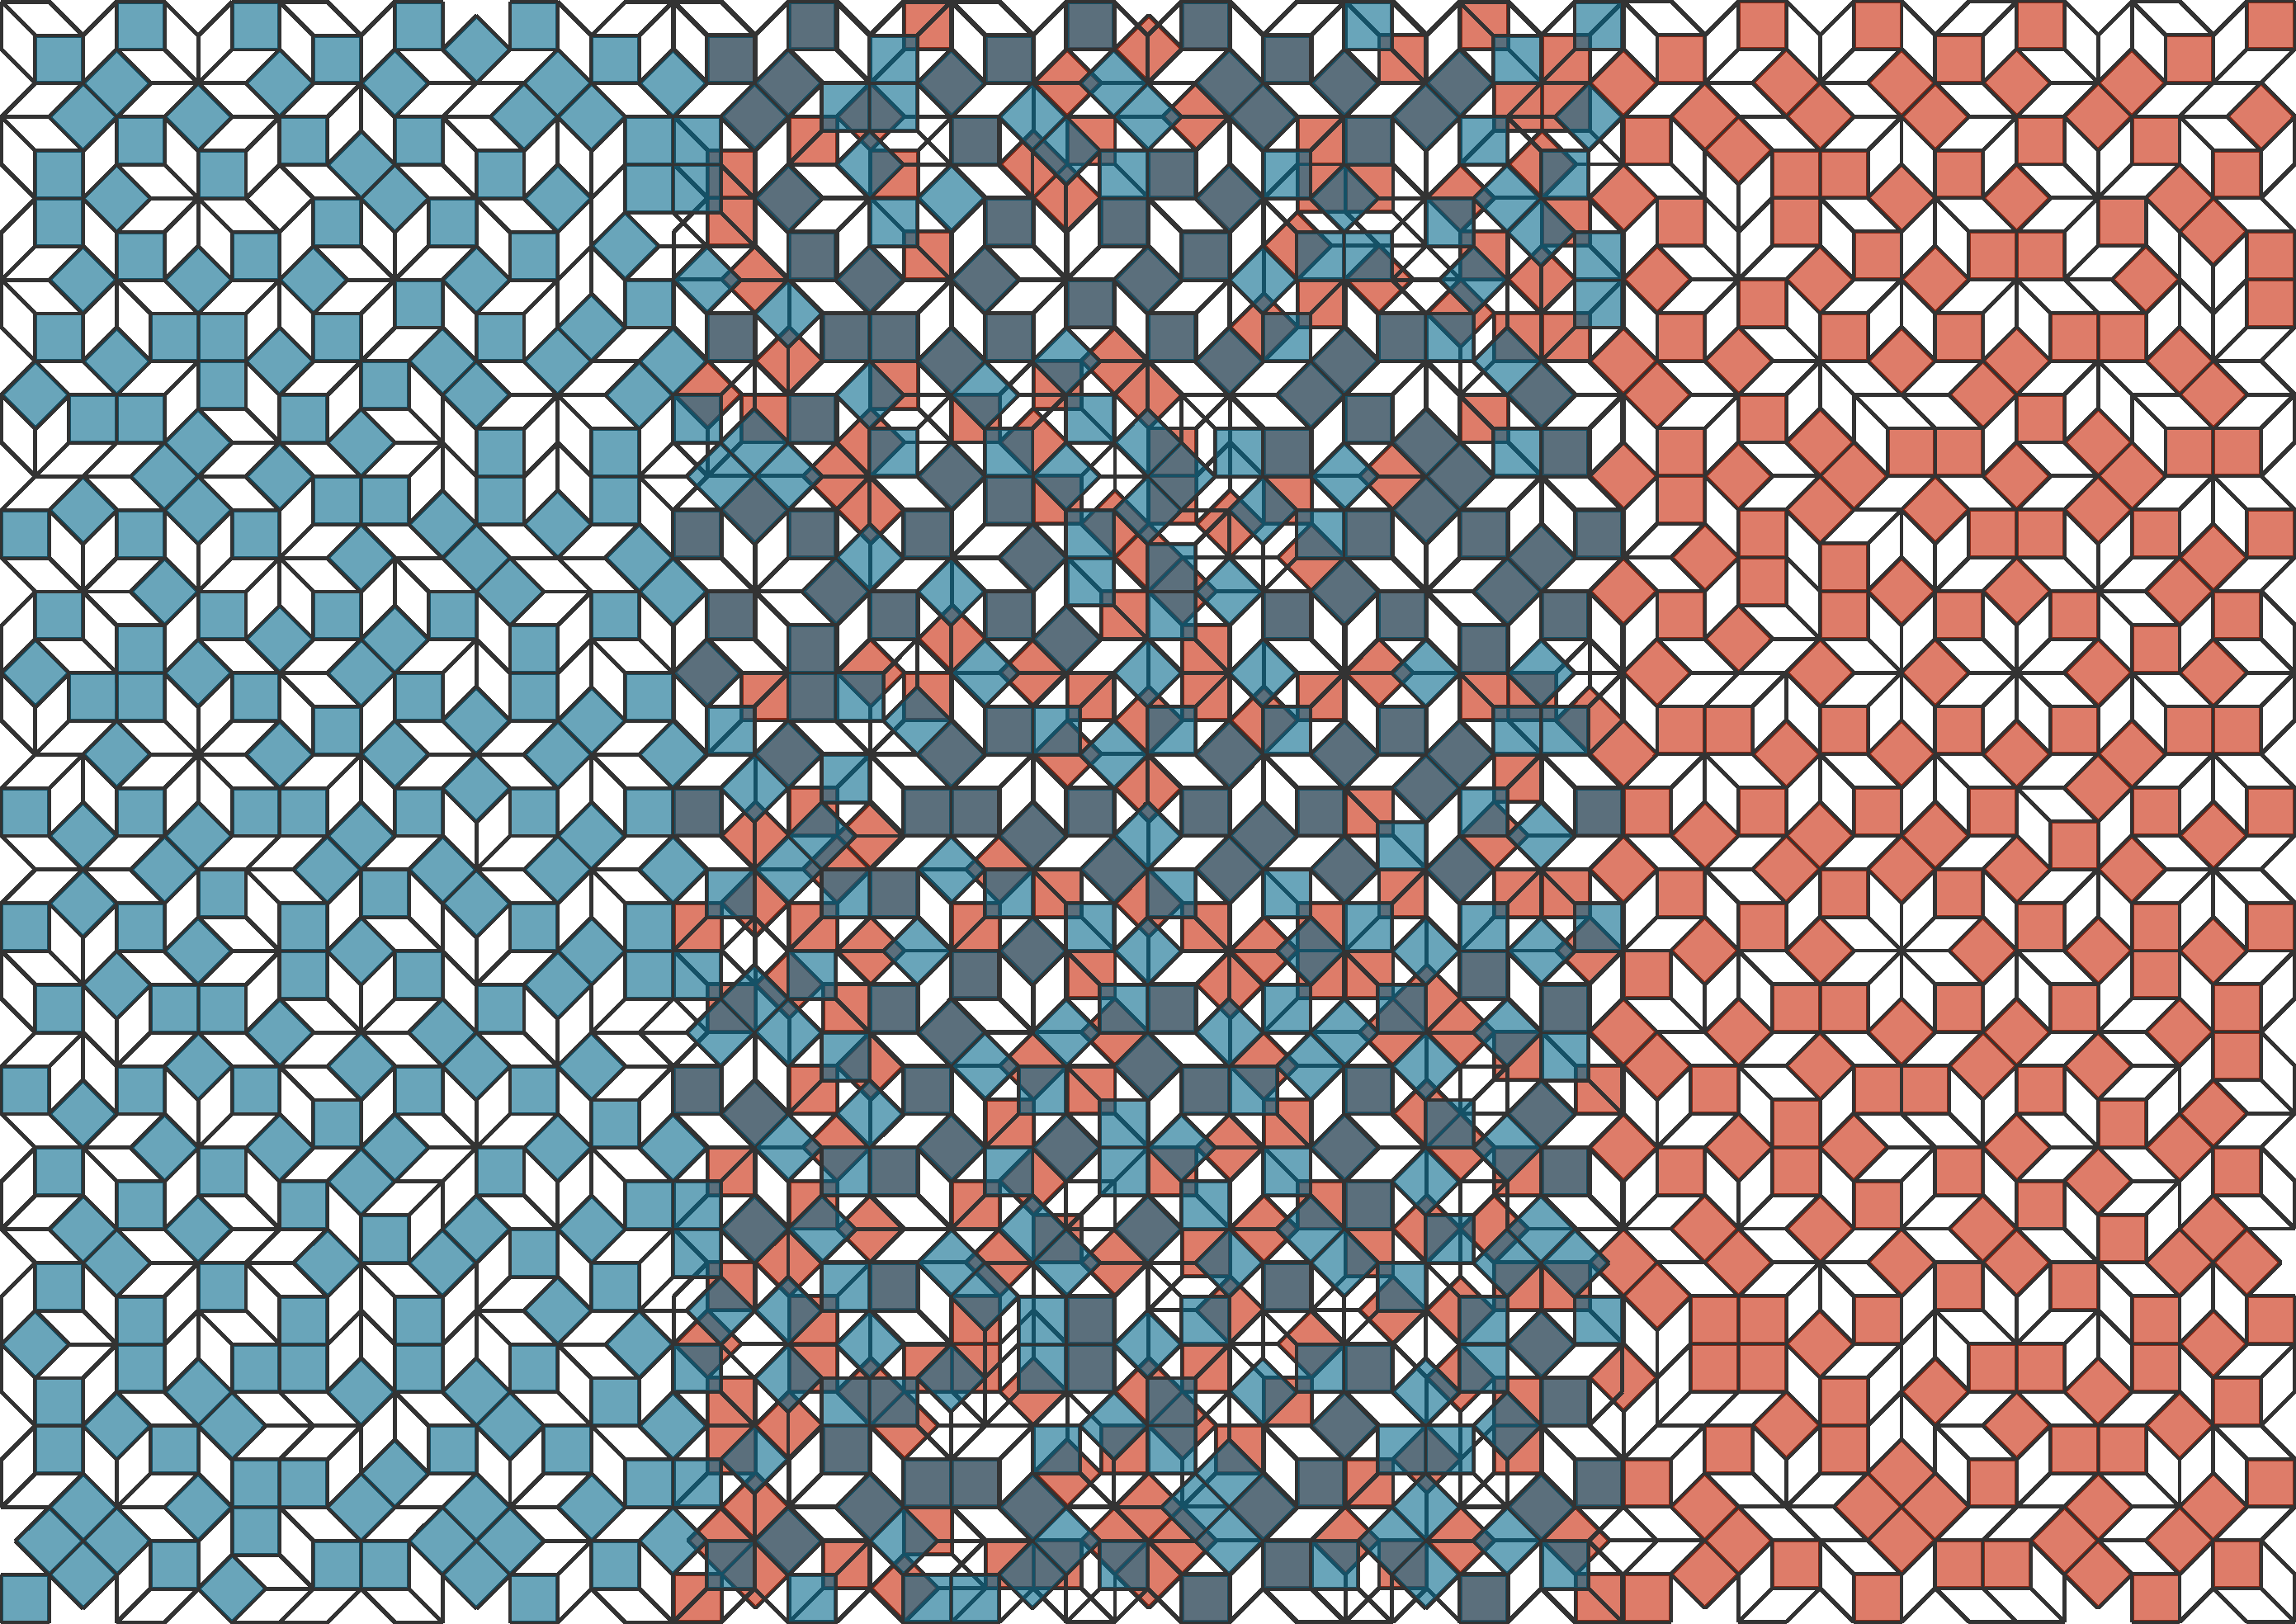
\includegraphics[width=.75\textwidth]{img/random.pdf}

$\to$ no overlap $\to$ no order}

\centering
\only<4>{
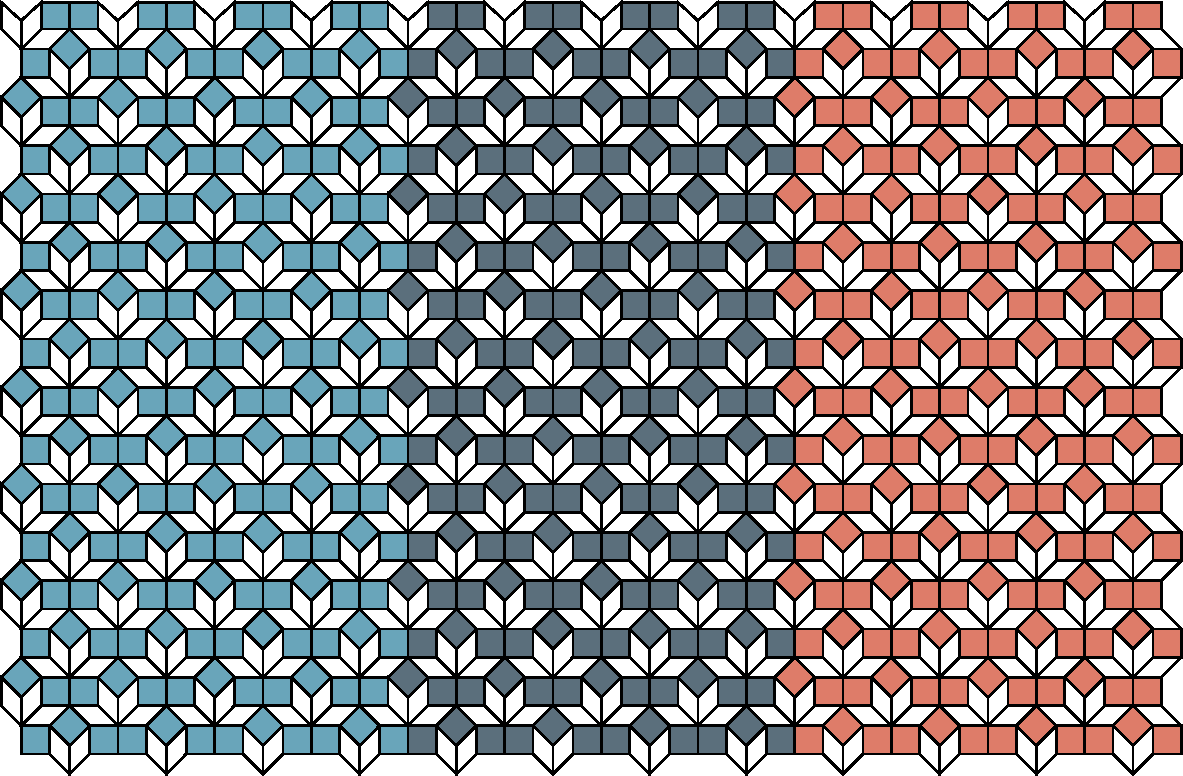
\includegraphics[width=.75\textwidth]{img/periodic.pdf}

Perfect long range order: periodic}

\only<5>{
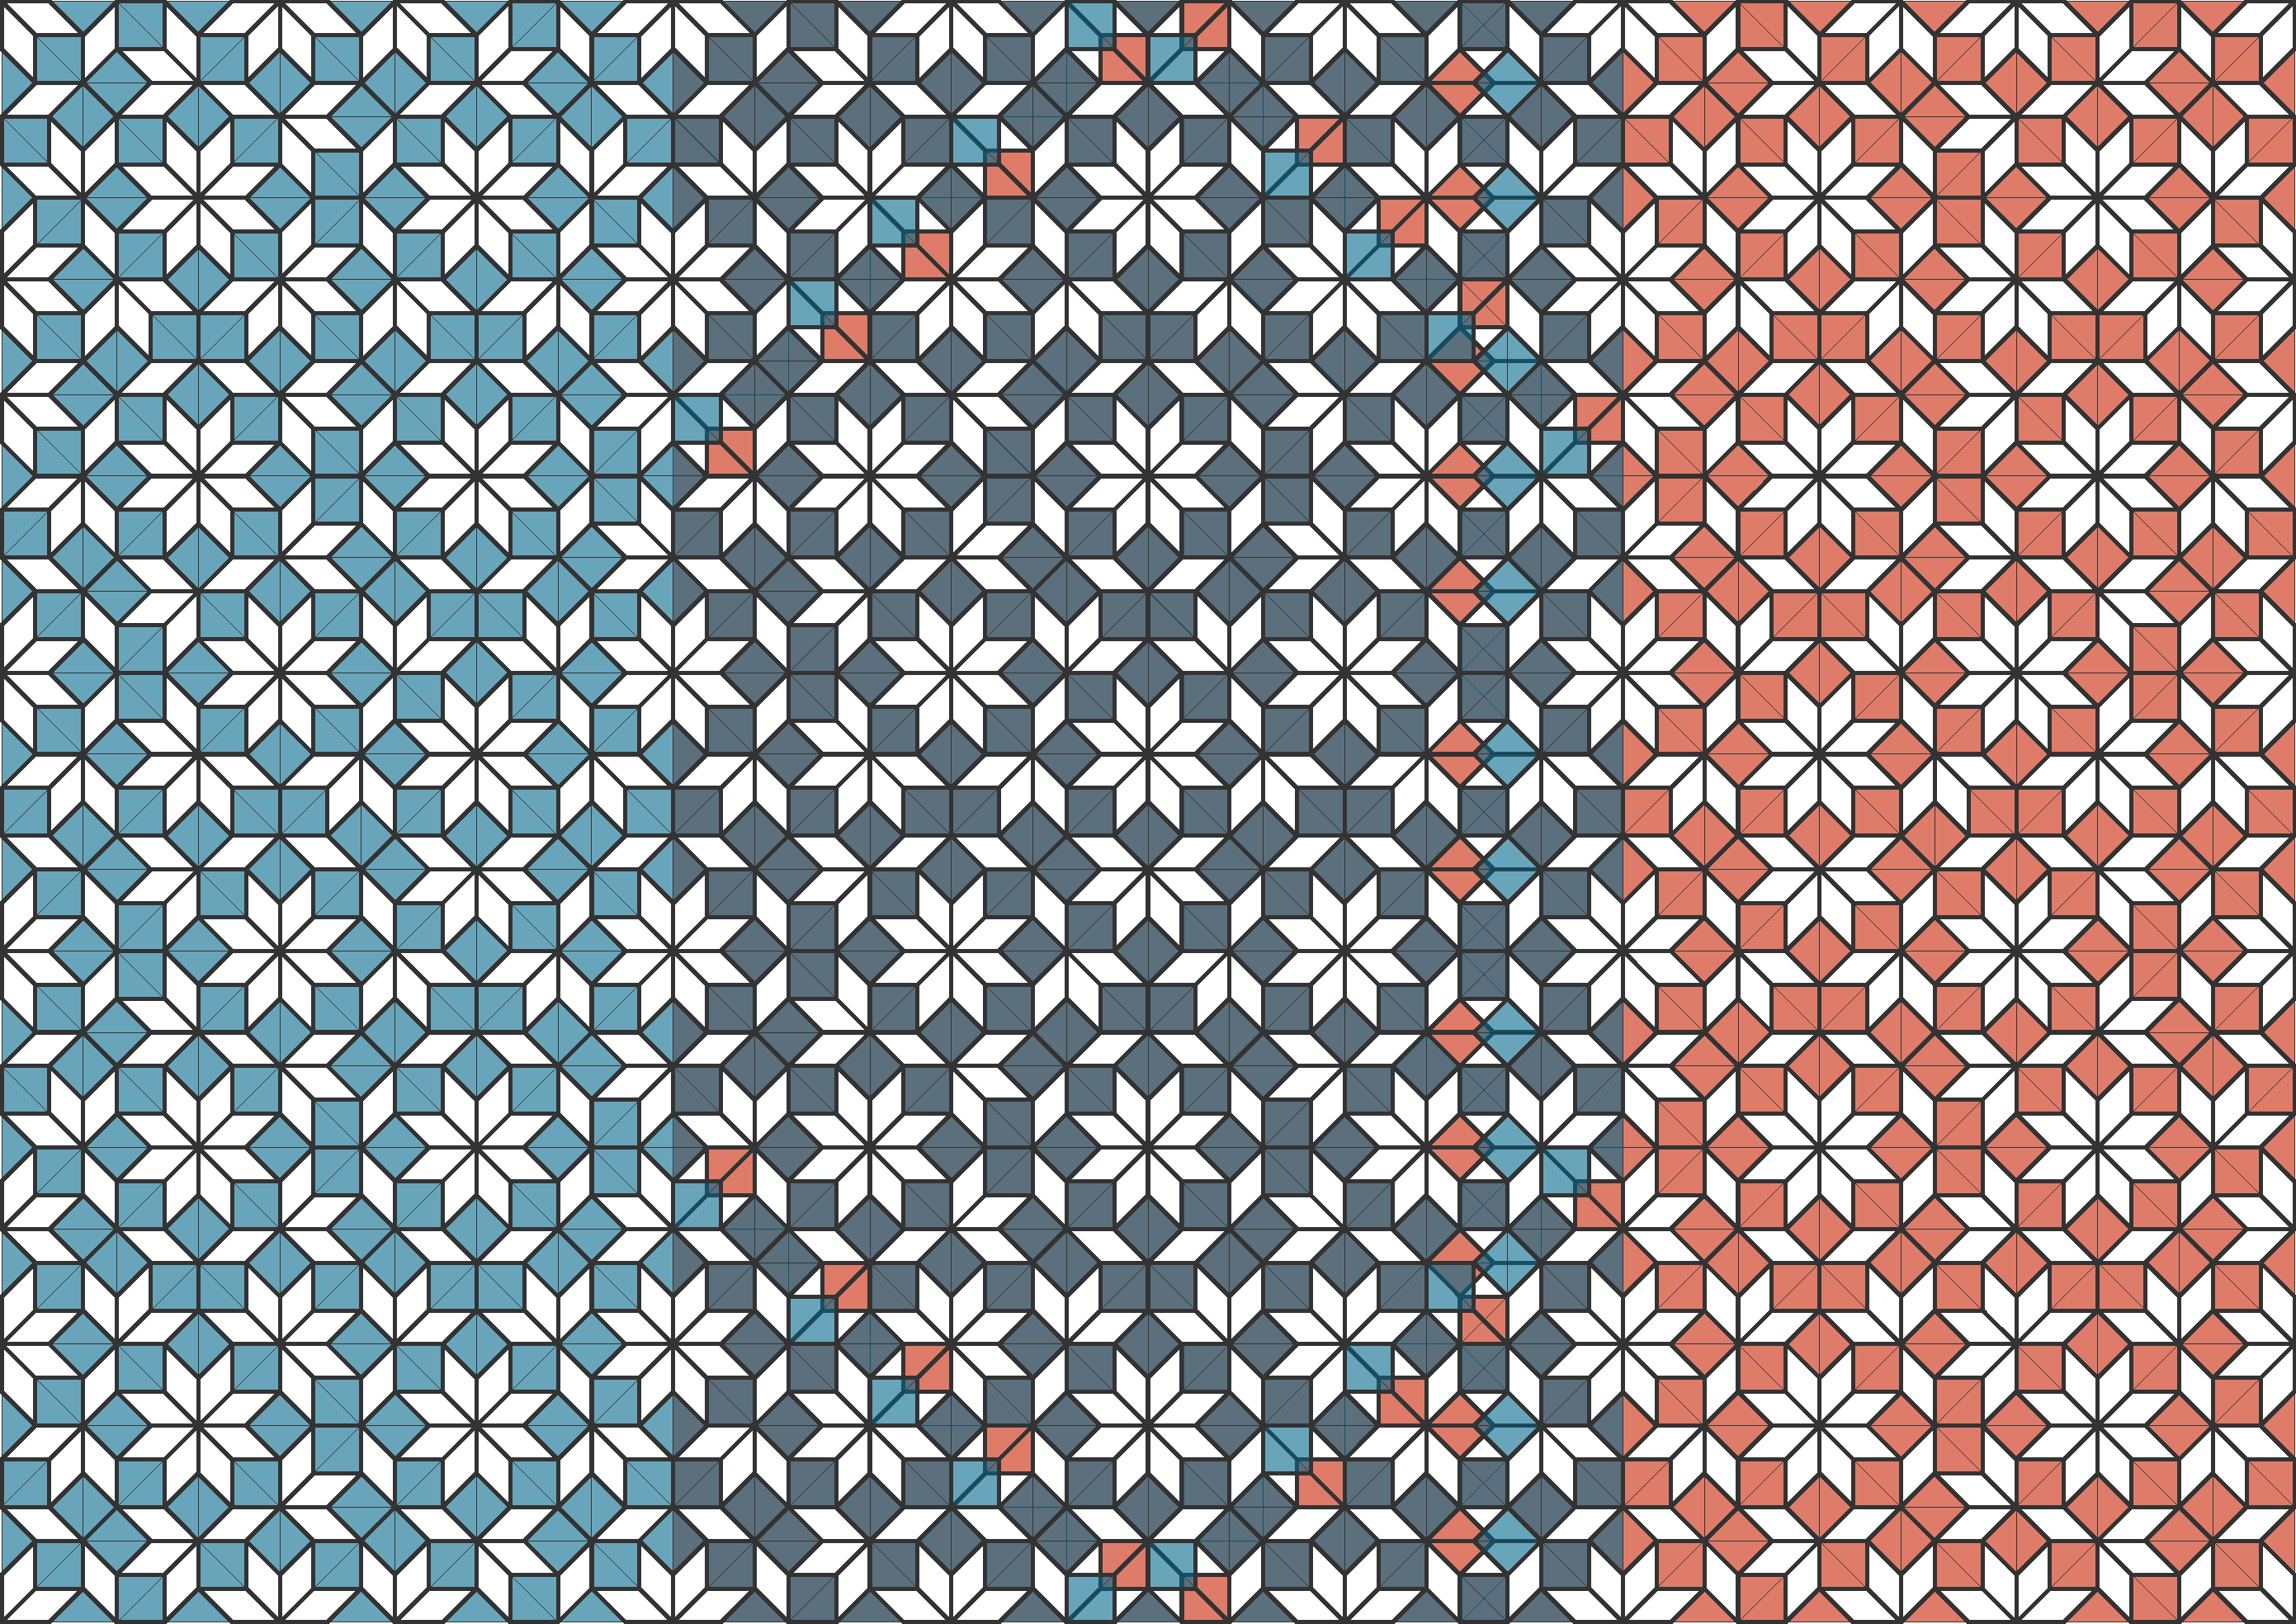
\includegraphics[width=.75\textwidth]{img/quasiperiodic.pdf}

Long range order: quasiperiodic 

\flushleft{(see Chap.\ 2 of [Grimm, Baake 13])}
}

\end{frame}

\begin{frame}{Real life examples}
\(
	\<{6cm}
		\centering
		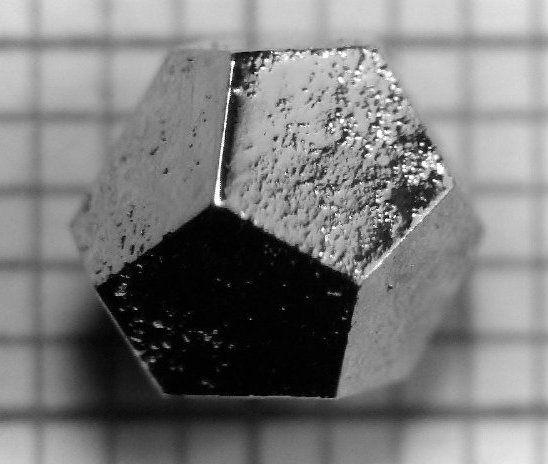
\includegraphics[scale=0.28]{img/homgzn.png}
		
		\ss{HoMgZn alloy in its icosahedral phase} \ss{(see \url{doi:10.1038/nmat1244})}
	\>
	\<{6cm}
		\centering
		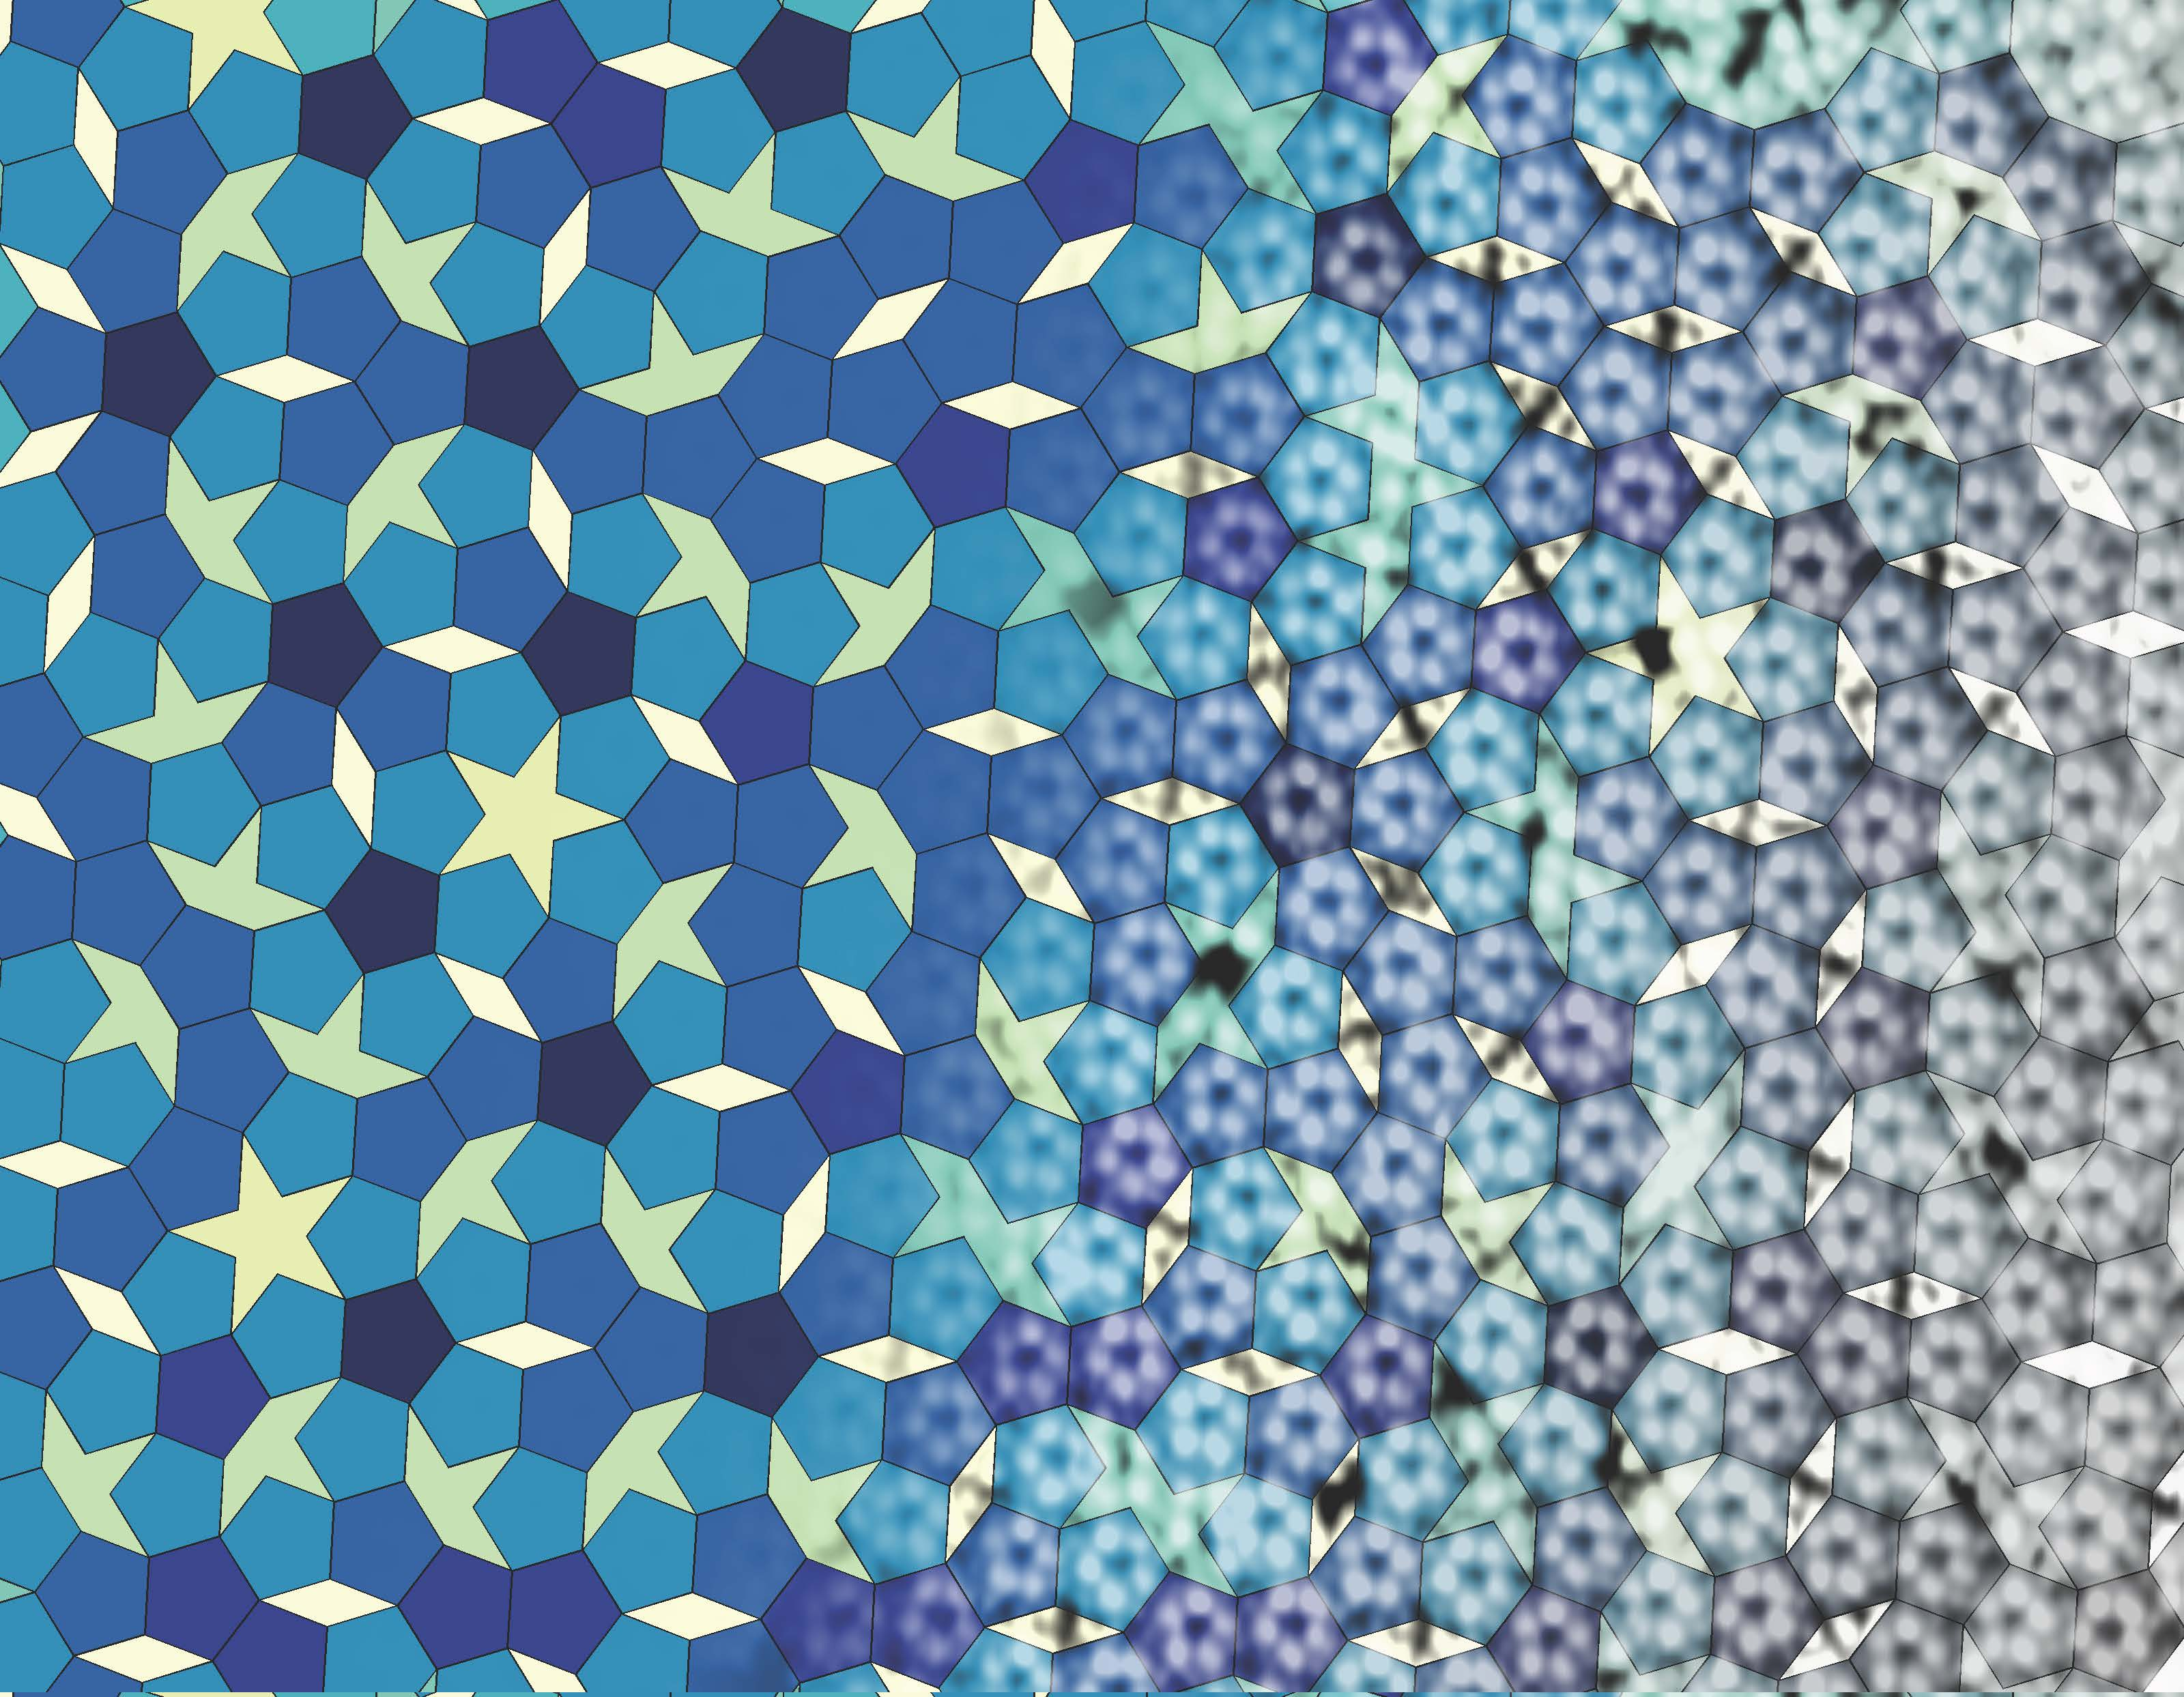
\includegraphics[scale=0.22]{img/wasio.jpg}
		
		\ss{A 2D hydrogen-bonded quasicrystal} \ss{(see \url{doi:10.1038/nature12993})}
	\>
\)

\begin{itemize}
	\item Numerous metallic and soft-matter quasicrystals have been synthetized
	\item only one natural example example is known: the Khatyrka meteorite (see \url{doi:10.1126/science.1170827 }). 
\end{itemize}
\end{frame}